\paragraph{}
Ze względu na architekturę aplikacji, klasy używane na CPU oddzielone są od klas karty graficznej. Oczywiście te drugie są klasami jedynie logicznie - ze względu na konieczność używania języka C w kodzie dla GPU. Ponieważ jednak obiekty są wygodną abstrakcją, będziemy z niej korzystać w całym programie.

\subsubsection{Klasy GPU}

\begin{figure}[h]
	\centering
	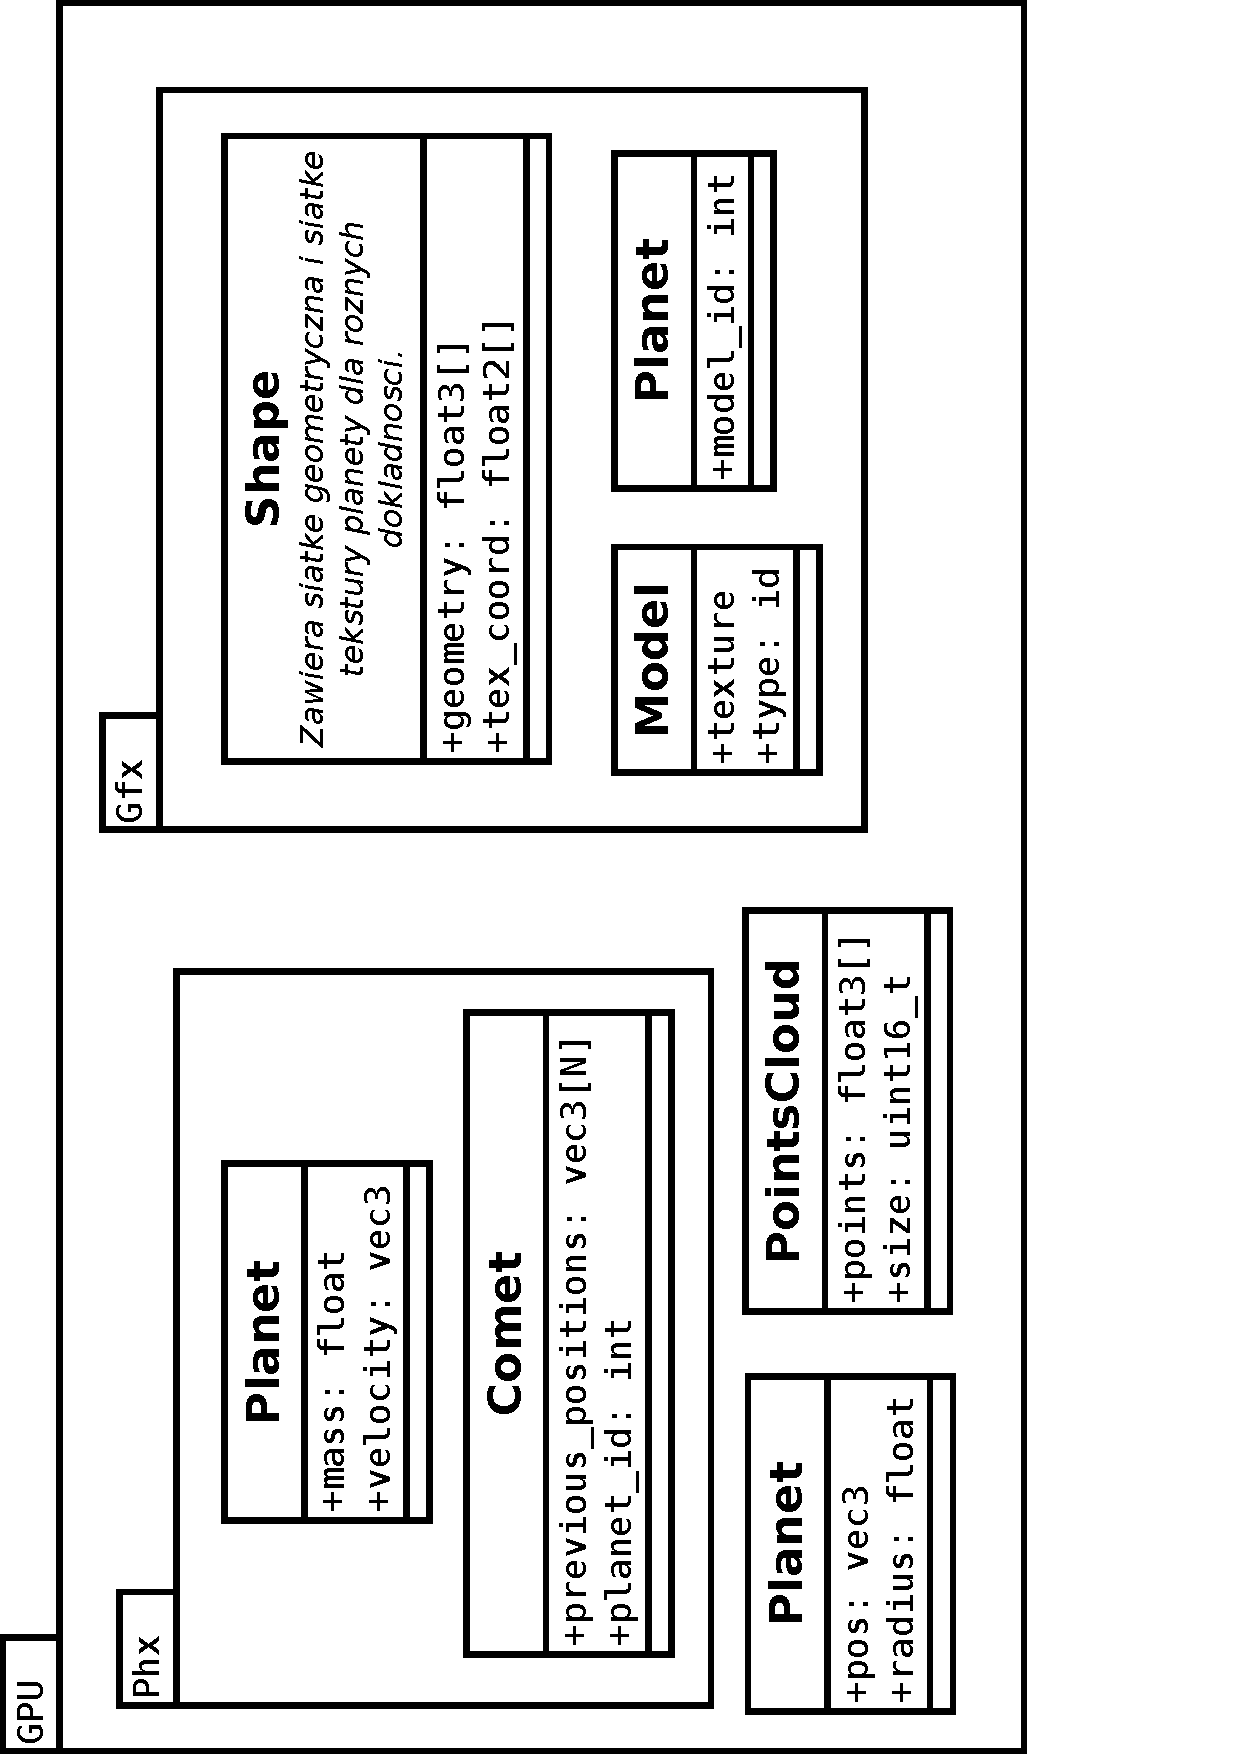
\includegraphics[angle=270,width=0.8\textwidth]{class_gpu.pdf}
	\caption{Diagram klas dla GPU}
	\label{fig:class_gpu}
\end{figure}

\paragraph{}
Struktury, z których będziemy korzystać na karcie graficznej, określone są na rysunku \ref{fig:class_gpu}. Ponieważ karta graficzna służy nam zarówno do wyświetlania danych, jak i do ich przetwarzania, wydzielone są na nim dwie przestrzenie nazw. Są to:
\begin{itemize}
	\item{Phx - do operacji fizycznych}
	\item{Gfx - do operacji graficznych}
\end{itemize}

\paragraph{}
Ponadto istnieje kilka struktur wspólnych dla obu częsci.

\paragraph{GPU::Planet} zawiera informacje, z których korzystaja zarówno wyświetlanie jak i fizyka. Jest to położenie planety oraz jej promień.
\paragraph{GPU::PointsCloud} reprezentuje chmurę cząstek - jest ona obliczana dla każdej widocznej komety przez moduł fizyczny.

\paragraph{}
Operacje fizyczne odbywać się będą z wykorzystaniem dwóch dodatkowych struktur.

\paragraph{GPU::Phx::Planet} to dodatkowe informacje o każdej planecie, które są potrzebne jedynie silnikowi fizycznemu. Należą do nich prędkość oraz masa.
\paragraph{GPU::Phx::Comet} stanowi dodatkową informację o planecie. Struktura ta istnieje tylko dla obiektów będących kometami. Zawiera kilka ostatnich pozycji oraz identyfikator planety.

\paragraph{}
Do wyświetlenia planet konieczne będą informacje o teksturach, oraz o siatkach każdej z planet.

\paragraph{GPU::Gfx::Planet} zawiera indeks modelu, czyli wyglądu planetu. Dwie planety mogą mieć ten sam model.
\paragraph{GPU::Gfx::Model} definiuje konkretny wygląd. Na tym poziomie będziemy rozróżniać zwykłe planety od gwiazd i komet.
\paragraph{GPU::Gfx::Shape} agreguje informację o siatce planety w 3D oraz odpowiadającej jej siatce na dwuwymiarowej teksturze.

\subsubsection{Klasy CPU}

\begin{figure}[ht!]
	\centering
	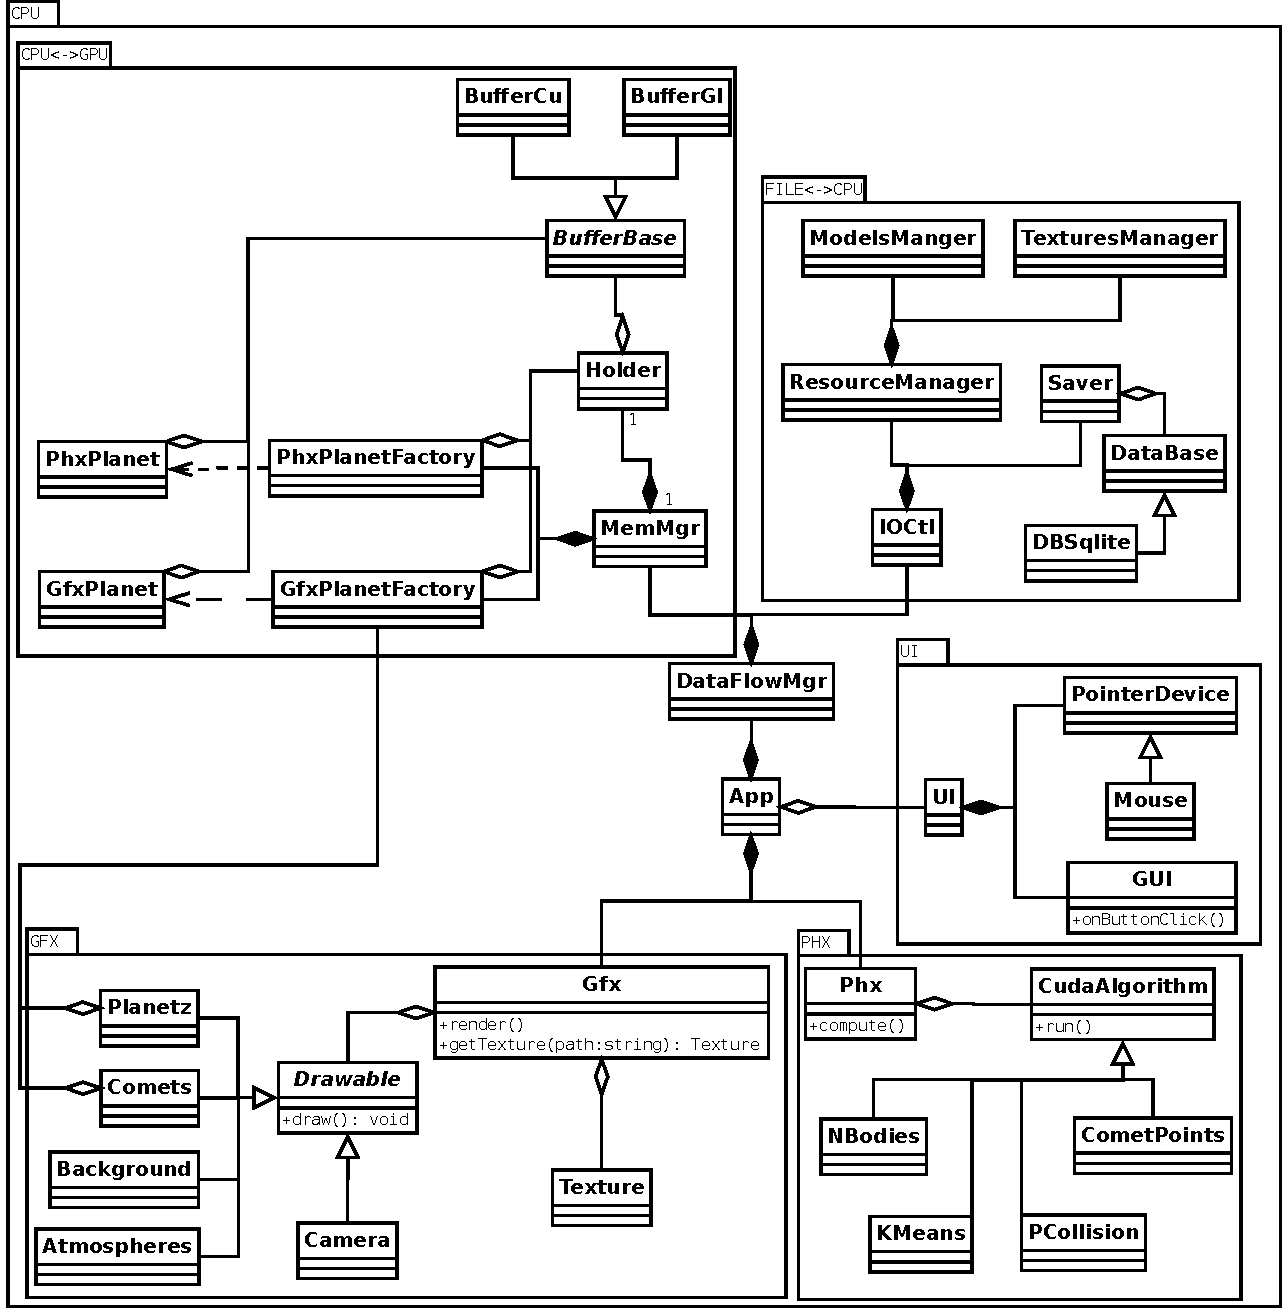
\includegraphics[angle=0,width=\textwidth]{class_cpu.pdf}
	\caption{Diagram klas dla CPU}
	\label{fig:class_cpu}
\end{figure}

\paragraph{}
Ta część klas przełoży się bezpośrednio na klasy znane z c++. Diagram klas znajduje się na rysunku \ref{fig:class_cpu}.

\paragraph{CPU::App} jest główną klasą, zarządzającą obiektami GFX, PHX, DataFlowMgr oraz UI. Tworzy je ona na początku działania programu.
\paragraph{CPU::GFX} odpowiada za wyświetlanie. Korzysta przy tym z biblioteki OpenGL.
\paragraph{CPU::PHX} uruchamia kernel'e CUDA, które przeprowadzają wszystkie obliczenia fizyczne.
\paragraph{CPU::DataFlowMgr} wykonuje wszystkie przepływy danych - pomiędzy RAM karty graficznej, RAM komputera oraz dyskiem twardym.
\paragraph{CPU::MemMgr} na zlecenie DataFlowMgr'a przenosi dane pomiędzy kartą graficzną a RAM.
\paragraph{CPU::IOCtl} na zlecenie DataFlowMgr'a przenosi dane pomiędzy RAM a dyskiem twardym.
\paragraph{CPU::UI} odpowiada za całość interakcji z użytkownikiem.
\paragraph{CPU::GUI}, czyli graficzny interfejs użytkownika. Obsługa okienek.
\paragraph{CPU::InputDev} obsługuje klawiaturę i mysz.
\paragraph{CPU::PlanetPicker} służy do określania, która planeta została zaznaczona.
